


\tikzset{every picture/.style={line width=0.75pt}} %set default line width to 0.75pt        

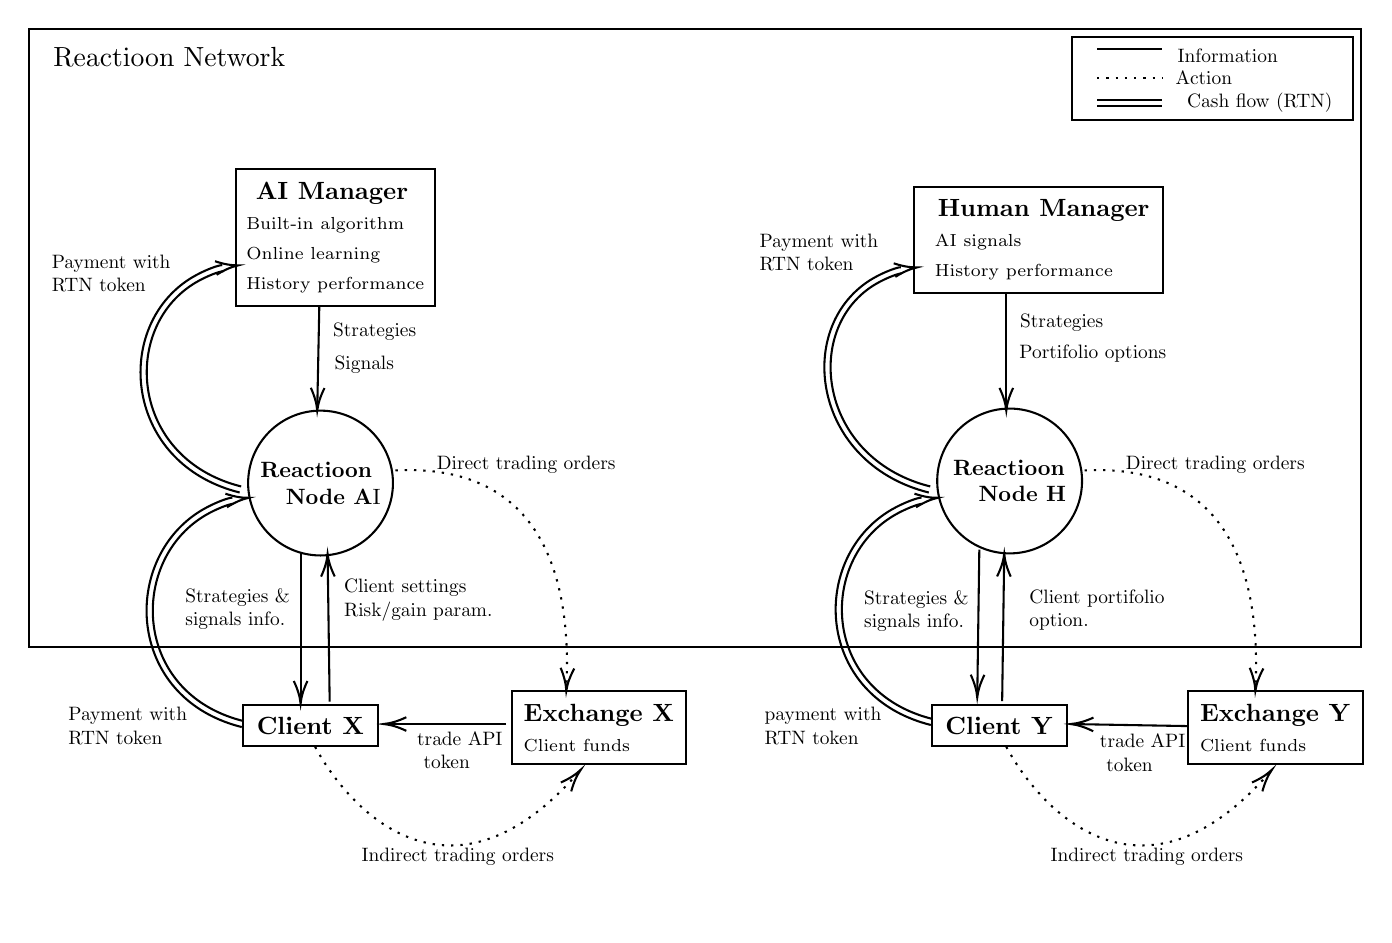
\begin{tikzpicture}[x=0.75pt,y=0.75pt,yscale=-1,xscale=1]
%uncomment if require: \path (0,464.1999969482422); %set diagram left start at 0, and has height of 464.1999969482422

%Shape: Rectangle [id:dp839607811925092] 
\draw   (16.3,16.2) -- (658.3,16.2) -- (658.3,314.2) -- (16.3,314.2) -- cycle ;
%Straight Lines [id:da3953078356379509] 
\draw    (156.3,150.2) -- (155.34,198.2) ;
\draw [shift={(155.3,200.2)}, rotate = 271.15] [color={rgb, 255:red, 0; green, 0; blue, 0 }  ][line width=0.75]    (10.93,-3.29) .. controls (6.95,-1.4) and (3.31,-0.3) .. (0,0) .. controls (3.31,0.3) and (6.95,1.4) .. (10.93,3.29)   ;

%Straight Lines [id:da5714023605084257] 
\draw    (246.3,351.2) -- (189.3,351.2) ;
\draw [shift={(187.3,351.2)}, rotate = 360] [color={rgb, 255:red, 0; green, 0; blue, 0 }  ][line width=0.75]    (10.93,-3.29) .. controls (6.95,-1.4) and (3.31,-0.3) .. (0,0) .. controls (3.31,0.3) and (6.95,1.4) .. (10.93,3.29)   ;

%Straight Lines [id:da41026468235715097] 
\draw    (161.3,340.4) -- (160.33,271.2) ;
\draw [shift={(160.3,269.2)}, rotate = 449.2] [color={rgb, 255:red, 0; green, 0; blue, 0 }  ][line width=0.75]    (10.93,-3.29) .. controls (6.95,-1.4) and (3.31,-0.3) .. (0,0) .. controls (3.31,0.3) and (6.95,1.4) .. (10.93,3.29)   ;

%Curve Lines [id:da9188372161085148] 
\draw  [dash pattern={on 0.84pt off 2.51pt}]  (193,229) .. controls (247.03,226.21) and (278.98,257.88) .. (275.36,334.05) ;
\draw [shift={(275.3,335.2)}, rotate = 272.97] [color={rgb, 255:red, 0; green, 0; blue, 0 }  ][line width=0.75]    (10.93,-3.29) .. controls (6.95,-1.4) and (3.31,-0.3) .. (0,0) .. controls (3.31,0.3) and (6.95,1.4) .. (10.93,3.29)   ;

%Curve Lines [id:da6611499345431215] 
\draw    (118.94,352.66) .. controls (94.86,346.64) and (80.76,330.95) .. (75.48,313.17) .. controls (73.99,308.15) and (73.2,302.97) .. (73.09,297.78) .. controls (73.09,297.38) and (73.08,296.99) .. (73.08,296.59) .. controls (73.08,277.29) and (82.51,258.18) .. (100.08,247.93) .. controls (105.93,244.51) and (112.7,242.08) .. (114.44,242.12)(119.66,349.74) .. controls (96.83,344.04) and (83.37,329.2) .. (78.35,312.32) .. controls (76.94,307.56) and (76.19,302.64) .. (76.09,297.72) .. controls (76.09,297.34) and (76.08,296.96) .. (76.08,296.59) .. controls (76.08,278.33) and (84.95,260.23) .. (101.59,250.52) .. controls (107.14,247.28) and (113.54,244.98) .. (114.89,245.1) ;
\draw [shift={(122.3,242.2)}, rotate = 533.23] [color={rgb, 255:red, 0; green, 0; blue, 0 }  ][line width=0.75]    (10.93,-3.29) .. controls (6.95,-1.4) and (3.31,-0.3) .. (0,0) .. controls (3.31,0.3) and (6.95,1.4) .. (10.93,3.29)   ;

%Curve Lines [id:da6558944188118099] 
\draw    (117.94,239.66) .. controls (92.68,233.34) and (77.79,216.52) .. (72.44,197.85) .. controls (71.26,193.75) and (70.54,189.55) .. (70.28,185.36) .. controls (70.21,184.14) and (70.17,182.92) .. (70.17,181.71) .. controls (70.17,163.45) and (78.74,145.72) .. (95.16,135.95) .. controls (100.92,132.53) and (107.65,130.08) .. (109.53,130.09)(118.66,236.74) .. controls (94.65,230.74) and (80.42,214.8) .. (75.32,197.03) .. controls (74.2,193.13) and (73.53,189.15) .. (73.28,185.17) .. controls (73.2,184.02) and (73.17,182.86) .. (73.17,181.71) .. controls (73.17,164.5) and (81.2,147.75) .. (96.69,138.53) .. controls (102.14,135.29) and (108.51,132.99) .. (109.98,133.07) ;
\draw [shift={(117.3,130.2)}, rotate = 533.23] [color={rgb, 255:red, 0; green, 0; blue, 0 }  ][line width=0.75]    (10.93,-3.29) .. controls (6.95,-1.4) and (3.31,-0.3) .. (0,0) .. controls (3.31,0.3) and (6.95,1.4) .. (10.93,3.29)   ;

%Curve Lines [id:da7197337789763143] 
\draw  [dash pattern={on 0.84pt off 2.51pt}]  (154.3,362.2) .. controls (173.2,397.02) and (221.81,442.74) .. (281.4,374.24) ;
\draw [shift={(282.3,373.2)}, rotate = 490.6] [color={rgb, 255:red, 0; green, 0; blue, 0 }  ][line width=0.75]    (10.93,-3.29) .. controls (6.95,-1.4) and (3.31,-0.3) .. (0,0) .. controls (3.31,0.3) and (6.95,1.4) .. (10.93,3.29)   ;

%Straight Lines [id:da7501707624311069] 
\draw    (487.3,144.2) -- (487.3,198.2) ;
\draw [shift={(487.3,200.2)}, rotate = 270] [color={rgb, 255:red, 0; green, 0; blue, 0 }  ][line width=0.75]    (10.93,-3.29) .. controls (6.95,-1.4) and (3.31,-0.3) .. (0,0) .. controls (3.31,0.3) and (6.95,1.4) .. (10.93,3.29)   ;

%Straight Lines [id:da11297405436688912] 
\draw    (575.3,352.2) -- (520.3,351.24) ;
\draw [shift={(518.3,351.2)}, rotate = 361.01] [color={rgb, 255:red, 0; green, 0; blue, 0 }  ][line width=0.75]    (10.93,-3.29) .. controls (6.95,-1.4) and (3.31,-0.3) .. (0,0) .. controls (3.31,0.3) and (6.95,1.4) .. (10.93,3.29)   ;

%Straight Lines [id:da9530469398494208] 
\draw    (485.3,340.2) -- (486.27,271.2) ;
\draw [shift={(486.3,269.2)}, rotate = 450.81] [color={rgb, 255:red, 0; green, 0; blue, 0 }  ][line width=0.75]    (10.93,-3.29) .. controls (6.95,-1.4) and (3.31,-0.3) .. (0,0) .. controls (3.31,0.3) and (6.95,1.4) .. (10.93,3.29)   ;

%Curve Lines [id:da6669727888364709] 
\draw  [dash pattern={on 0.84pt off 2.51pt}]  (525,229) .. controls (579.03,226.21) and (610.98,257.88) .. (607.36,334.05) ;
\draw [shift={(607.3,335.2)}, rotate = 272.97] [color={rgb, 255:red, 0; green, 0; blue, 0 }  ][line width=0.75]    (10.93,-3.29) .. controls (6.95,-1.4) and (3.31,-0.3) .. (0,0) .. controls (3.31,0.3) and (6.95,1.4) .. (10.93,3.29)   ;

%Curve Lines [id:da6929077991045711] 
\draw    (450.94,351.66) .. controls (426.58,345.57) and (412.42,329.71) .. (407.29,311.85) .. controls (405.93,307.09) and (405.2,302.19) .. (405.1,297.3) .. controls (405.09,296.88) and (405.08,296.47) .. (405.08,296.05) .. controls (405.08,276.94) and (414.51,258.04) .. (432.08,247.87) .. controls (437.94,244.49) and (444.7,242.07) .. (446.45,242.11)(451.66,348.74) .. controls (428.56,342.97) and (415.05,327.99) .. (410.18,311.02) .. controls (408.88,306.51) and (408.19,301.87) .. (408.1,297.23) .. controls (408.09,296.84) and (408.08,296.45) .. (408.08,296.05) .. controls (408.08,277.99) and (416.95,260.09) .. (433.58,250.47) .. controls (439.13,247.26) and (445.54,244.98) .. (446.89,245.09) ;
\draw [shift={(454.3,242.2)}, rotate = 533.23] [color={rgb, 255:red, 0; green, 0; blue, 0 }  ][line width=0.75]    (10.93,-3.29) .. controls (6.95,-1.4) and (3.31,-0.3) .. (0,0) .. controls (3.31,0.3) and (6.95,1.4) .. (10.93,3.29)   ;

%Curve Lines [id:da46112590181388846] 
\draw    (449.94,239.66) .. controls (423.51,233.05) and (407.61,215.09) .. (401.97,195.59) .. controls (401.05,192.4) and (400.4,189.18) .. (400.03,185.95) .. controls (399.77,183.73) and (399.64,181.5) .. (399.64,179.29) .. controls (399.64,162) and (407.53,145.57) .. (423.1,136.49) .. controls (428.56,133.31) and (434.97,131.03) .. (436.48,131.11)(450.66,236.74) .. controls (425.47,230.45) and (410.24,213.37) .. (404.85,194.75) .. controls (403.98,191.73) and (403.36,188.67) .. (403.01,185.61) .. controls (402.76,183.5) and (402.64,181.39) .. (402.64,179.29) .. controls (402.64,163.07) and (409.98,147.61) .. (424.62,139.09) .. controls (429.77,136.08) and (435.82,133.94) .. (436.95,134.08) ;
\draw [shift={(444.3,131.2)}, rotate = 533.23] [color={rgb, 255:red, 0; green, 0; blue, 0 }  ][line width=0.75]    (10.93,-3.29) .. controls (6.95,-1.4) and (3.31,-0.3) .. (0,0) .. controls (3.31,0.3) and (6.95,1.4) .. (10.93,3.29)   ;

%Curve Lines [id:da8354818907327548] 
\draw  [dash pattern={on 0.84pt off 2.51pt}]  (487.3,362.2) .. controls (506.2,397.02) and (554.81,442.74) .. (614.4,374.24) ;
\draw [shift={(615.3,373.2)}, rotate = 490.6] [color={rgb, 255:red, 0; green, 0; blue, 0 }  ][line width=0.75]    (10.93,-3.29) .. controls (6.95,-1.4) and (3.31,-0.3) .. (0,0) .. controls (3.31,0.3) and (6.95,1.4) .. (10.93,3.29)   ;

%Straight Lines [id:da8770926699692774] 
\draw    (147.3,268.2) -- (147.3,339.4) ;
\draw [shift={(147.3,341.4)}, rotate = 270] [color={rgb, 255:red, 0; green, 0; blue, 0 }  ][line width=0.75]    (10.93,-3.29) .. controls (6.95,-1.4) and (3.31,-0.3) .. (0,0) .. controls (3.31,0.3) and (6.95,1.4) .. (10.93,3.29)   ;

%Straight Lines [id:da36937072037759555] 
\draw    (474.3,267.2) -- (473.33,336.4) ;
\draw [shift={(473.3,338.4)}, rotate = 270.8] [color={rgb, 255:red, 0; green, 0; blue, 0 }  ][line width=0.75]    (10.93,-3.29) .. controls (6.95,-1.4) and (3.31,-0.3) .. (0,0) .. controls (3.31,0.3) and (6.95,1.4) .. (10.93,3.29)   ;

%Shape: Rectangle [id:dp03825033305531944] 
\draw   (518.9,20) -- (654.3,20) -- (654.3,60) -- (518.9,60) -- cycle ;
%Straight Lines [id:da5606203321141707] 
\draw    (531,26) -- (562.3,26) ;


%Straight Lines [id:da21375108102279738] 
\draw  [dash pattern={on 0.84pt off 2.51pt}]  (531,40) -- (562.3,40) ;


%Straight Lines [id:da15988012489637837] 
\draw    (531,50.5) -- (562.3,50.5)(531,53.5) -- (562.3,53.5) ;



% Text Node
\draw    (249,335.5) -- (333,335.5) -- (333,370.5) -- (249,370.5) -- cycle  ;
\draw (291,353) node [scale=0.9] [align=left] {\textbf{Exchange X}\\{\scriptsize Client funds}};
% Text Node
\draw    (119.5,342) -- (184.5,342) -- (184.5,362) -- (119.5,362) -- cycle  ;
\draw (152,352) node [scale=0.9] [align=left] {\textbf{ Client X }};
% Text Node
\draw    (116,84) -- (212,84) -- (212,150) -- (116,150) -- cycle  ;
\draw (164,117) node [scale=0.9] [align=left] {\textbf{ AI Manager}\\{\scriptsize  Built-in algorithm}\\{\scriptsize  Online learning}\\{\scriptsize  History performance}};
% Text Node
\draw    (156.9, 235.1) circle [x radius= 34.89, y radius= 34.89]   ;
\draw (156.9,235.1) node [scale=0.8] [align=left] {\textbf{Reactioon}\\\textbf{ \ \ Node A}I};
% Text Node
\draw (84,30) node  [align=left] {Reactioon Network};
% Text Node
\draw (224,364) node [scale=0.7] [align=left] {trade API \\ \ token};
% Text Node
\draw (183,162) node [scale=0.7] [align=left] {Strategies};
% Text Node
\draw (178,178) node [scale=0.7] [align=left] {Signals};
% Text Node
\draw (204,296) node [scale=0.7] [align=left] {Client settings\\Risk/gain param.\\};
% Text Node
\draw (64,352) node [scale=0.7] [align=left] {Payment with\\RTN token};
% Text Node
\draw (56,134) node [scale=0.7] [align=left] {Payment with\\ RTN token};
% Text Node
\draw (256,226) node [scale=0.7] [align=left] {Direct trading orders};
% Text Node
\draw (223,415) node [scale=0.7] [align=left] {Indirect trading orders};
% Text Node
\draw    (575,335.5) -- (659,335.5) -- (659,370.5) -- (575,370.5) -- cycle  ;
\draw (617,353) node [scale=0.9] [align=left] {\textbf{Exchange Y}\\{\scriptsize Client funds}};
% Text Node
\draw    (451.5,342) -- (516.5,342) -- (516.5,362) -- (451.5,362) -- cycle  ;
\draw (484,352) node [scale=0.9] [align=left] {\textbf{ Client Y }};
% Text Node
\draw    (443,92.5) -- (563,92.5) -- (563,143.5) -- (443,143.5) -- cycle  ;
\draw (503,118) node [scale=0.9] [align=left] {\textbf{ Human Manager }\\{\scriptsize  \ AI signals}\\{\scriptsize  \ History performance}};
% Text Node
\draw    (488.9, 234.1) circle [x radius= 34.89, y radius= 34.89]   ;
\draw (488.9,234.1) node [scale=0.8] [align=left] {\textbf{Reactioon}\\\textbf{ \ \ Node H}};
% Text Node
\draw (514,158) node [scale=0.7] [align=left] {Strategies};
% Text Node
\draw (529,173) node [scale=0.7] [align=left] {Portifolio options};
% Text Node
\draw (531,301) node [scale=0.7] [align=left] {Client portifolio\\option.\\};
% Text Node
\draw (588,226) node [scale=0.7] [align=left] {Direct trading orders};
% Text Node
\draw (555,415) node [scale=0.7] [align=left] {Indirect trading orders};
% Text Node
\draw (399,352) node [scale=0.7] [align=left] {payment with\\RTN token};
% Text Node
\draw (397,124) node [scale=0.7] [align=left] {Payment with\\ RTN token};
% Text Node
\draw (117,306) node [scale=0.7] [align=left] {Strategies \&\\signals info.\\\\};
% Text Node
\draw (444,307) node [scale=0.7] [align=left] {Strategies \&\\signals info.\\\\};
% Text Node
\draw (584,40) node [scale=0.7] [align=left] {Action };
% Text Node
\draw (594,29) node [scale=0.7] [align=left] {Information};
% Text Node
\draw (611,52) node [scale=0.7] [align=left] {Cash flow (RTN) };
% Text Node
\draw (553,365) node [scale=0.7] [align=left] {trade API \\ \ token};


\end{tikzpicture}
